\documentclass[11pt]{article}
\usepackage[letterpaper]{geometry}
\usepackage{times}
\usepackage{verbatim}
\usepackage{graphicx}
\usepackage{float}
\usepackage{fullwidth}
\usepackage{amsmath}
\usepackage{amssymb}
\usepackage{hyperref}
\graphicspath{{Images/}}
\title{ENGR-241 Analog Computer Lab}
\author{Jeremy Munson, Lauren Speirs \& Andrew Henrikson}
\geometry{top=.8in, bottom=.8in, left=.8in, right=.8in}

\setlength{\parindent}{0em}
\setlength{\parskip}{.5em}
\begin{document}
	\maketitle
	\subsection*{Overview}
	For this lab, we became familiar with the AMF analog computer. We produced a few output signals and explored how the analog computer was built. We then designed a new analog computer with fewer components that produced the same effects. The instructions include finding: f=a(b-10c) using the sum/difference module and to output the integral of the input using the integrating module. We then describe the purpose of the SET and 1.0 SEC---CONT functions. Lastly, we design new circuits of just one summing/difference and one integrating amplifier to produce the same results, describe the designs, and state the advantages and disadvantages of digital vs analog models. 
	\section*{Exploring the Analog Computer}
	
	\subsection*{Procedure}
	We demonstrated the ability of the AMF Computer to perform several math operations as described in the assignment requirements. The first test utilized the summing and difference Op Amp and the second showed the function of the integrating Op Amp. For each test, we measured the output with a fluke connected to the output jacks.
	
	\subsubsection*{Summing Amplifier: ($f=a(b-10c)$)}
	For this portion of the lab we supplied power to a 1x addition jack and a 10x subtraction jack and we set the potentiometer to a scaling factor of 1("a" value). The "b" value was set with the addition input and the "c" value was set with the subtracting input. We set the inputs at three different values and calculated the expected output for the chosen input values. The data is recorded is tabulated here.
	\begin{table}[h]
		\def\arraystretch{1.2}%
		\begin{tabular}{|l|l|l|l|l|l|l|}
			\hline
			Summing(a(b-10c))	& a(Scale) 		& b(1x in)	& c(-10x in)	& Output (Calculated)		& Output (Observed) 	& \% Diff				\\ \hline
			Test 1				& 1.0			& 0.454V	& 0.417V		& -3.72V					& -3.73V				&0.0722\%				\\ \hline
			Test 2				& 1.0			& 0.775V	& 0.671V		& -5.94V					& -5.96V				&0.3367\%				\\ \hline
			Test 3				& 1.0			& 1.004V	& 0.848V		& -7.48V					& -7.53V				&0.6684\%				\\ \hline
		\end{tabular}
	\end{table}
	
	\subsubsection*{Integrator ($f=\int$$f(t) {d}t$)}
	To perform the integration we connected a constant input to the integrating circuit and performed the tests over one second using the "1.0 SEC" mode described below to set our limits of integration. We performed three tests and compared the results to our calculated values. The data is tabulated here.
	\begin{table}[h]
		\def\arraystretch{1.2}%
		\begin{tabular}{|l|l|l|l|l|l|l|}
			\hline
			Integration(inverting)	& Input 		& Output(calculated)	& Output (Observed)	 		& \% Diff			\\ \hline
			Test 1					& 0.497V		& -0.497V				& -0.4V						&19.52\%			\\ \hline
			Test 2					& 1.009V		& -1.009V				& -0.87V					&13.78\%			\\ \hline
			Test 3					& 2.01V			& -2.001V				& -1.8V						&10.045\%			\\ \hline
		\end{tabular}
	\end{table}
	
	\subsection*{Exploring SET and 1.0 SEC---CONT Functions}
	By experiment (and suggestion from the professor) we discovered that the SET button "Sets" an initial condition. This is analogous to the +c when doing an integral, setting the initial value. Pressing the set button changes the current value of the integrator to match the voltage on the input.
	
	The 1.0 SEC---CONT toggle had 3 positions: 1.0 SEC (left), off (middle), and CONT (right). When in the off position the integrator holds the output at its current value. The 1.0 SEC position causes the analog computer to integrate the input signal for one second, then stop at the final value. This is equivalent to performing a definite integral from 0 to 1 second + c.
	The CONT position causes the integrator to run continuously, outputting the integral of the input waveform. If the definite integral of the input waveform over one period is not 0, then the integrator will eventually saturate in continuous mode.
	
	\subsection*{Competitor's Product Analysis}
	
	The Educational Computer runs off of a standard 60Hz power source and converts this to +/-15v dc for the op amps. 
	
	The analog computer has a variable input for each of its integrating and summing boards. This model has three summing and difference circuits and two integrating circuits. \\
	
	Each of the integrating Op Amps takes the inverse of an input voltage and integrates it with respect to time. There are three separate input plugs, two are will input the chosen value, and the third will amplify the input by a factor of ten. The initial conditions are set with the red button(labeled SET) which holds the voltage constant while adjusting the initial condition knob. For the tests we performed on this model sent the output values to a fluke, verifying the circuit functioned properly. There are two different modes of integration on the AMF Educational Computer, the computer has a switch that can select either continuous integration (labeled CONT) or an integration over 1 second(labeled 1.0 SEC.). We performed tests in both modes and had moderately accurate results considering the age of the equipment. For the tests we performed on this model, we connected the output to a fluke, verifying the circuit functioned properly. The data can be found in the "Integration" data tables above. \\
	
	All three of the summing and difference amplifiers take an input voltage and add or subtract there values depending on where the inputs are connected to the circuit. There are a total of 6 input plugs, three adding and three subtracting. Like the integrating input, there are two  that directly input in the chosen input voltage and one that scales the input by ten. This is true for both the adding and subtracting inputs. The circuit also has a potentiometer that scales the output between zero and one and it is adjusted by a knob on the computer. We performed multiple tests and had highly accurate results. For the tests we performed on this model, we connected the output to a fluke, verifying the circuit functioned properly. The data can be found in the "Summing" data tables above.
	
	\section*{Designing an Analog Computer}
	The analog computer was state-of-the-art in its day, but compared to today's digital models is somewhat clunky, simple, and inefficient. The new design attempts to produce the same results with fewer components, making the design more efficient.
	
	\begin{figure}[H]
		\centering
		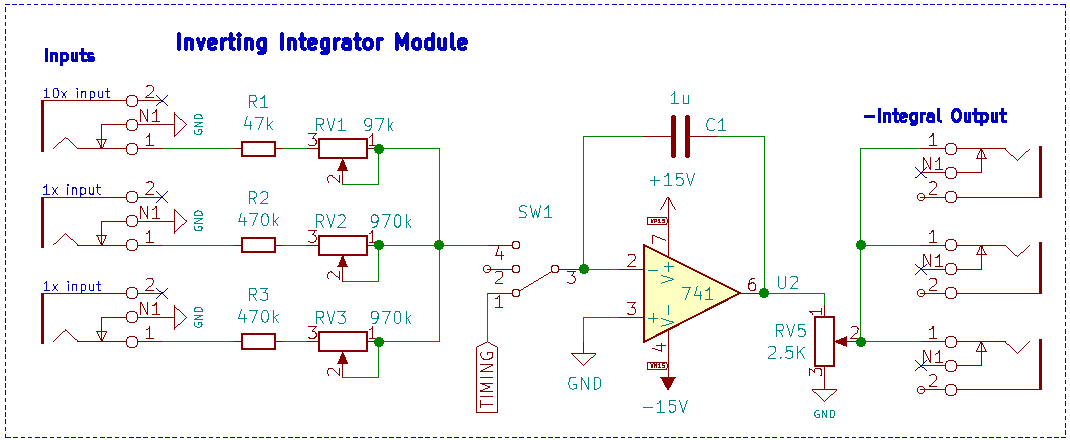
\includegraphics[width=6.5in]{images/schematic_integrator.png}
		
		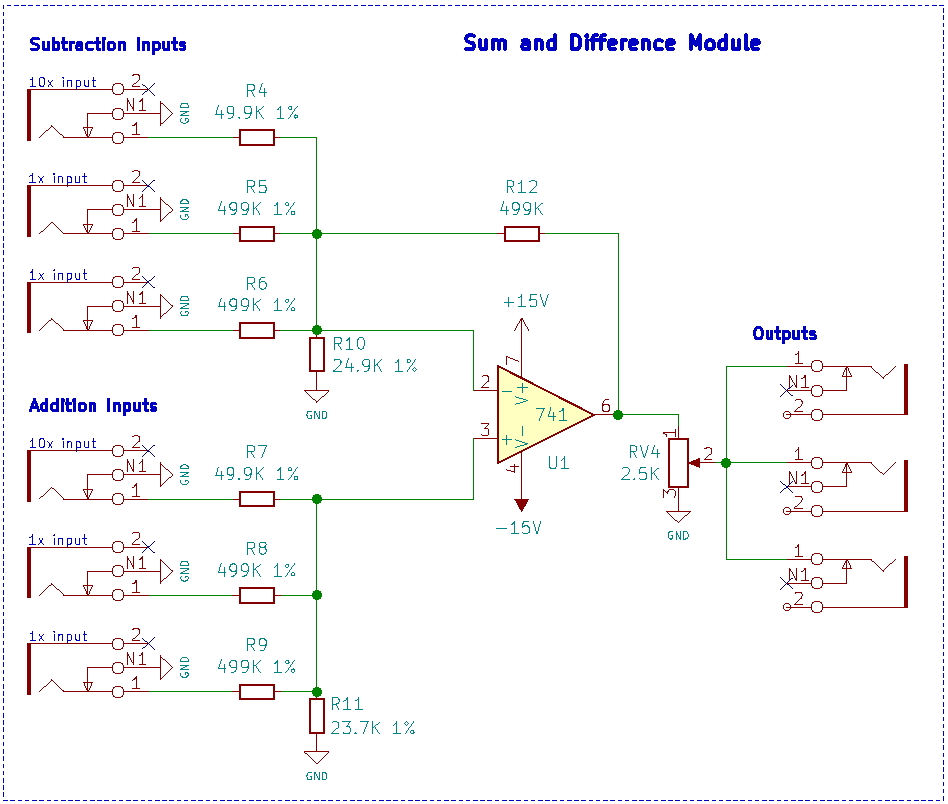
\includegraphics[width=6.5in]{images/schematic_sum_diff.png}
	\end{figure}

	
	\subsection*{Circuit Analysis}
	The circuit we have designed is similar in functionality to the Analog Computer described above. Our design incorporates a single summing and difference Op Amp and a single integrating Op Amp. Each of the circuits has a 741 Op Amp that are supplied with a +/- 15V V supply, and they both have three or 6 input and output jacks.  The input jacks are connected to ground when not in use to prevent spurious signals from interfering with the circuit. There are two "1x" inputs and one "10x" input for each circuit, similar to the AMF computer.
	
	The integrating circuit uses a feedback capacitor to perform the integration by charging and discharging as the input of the circuit changes. Resistor and Capacitance values were chosen to provide an output that is one times the integral (after calibration) and it is inverting because the feedback is negative. Large resistor values were chosen for the circuit to minimize the input current required, and to match the functionality of the competing product.
	
	The addition and subtraction sub-circuit takes the input voltages and uses the inverting and non-inverting terminals of the Op Amp to perform addition and subtraction. 
	
	\subsection*{Circuit Simulation}
	After creating our schematics we used KiCad/ngspice to simulate the circuits and verify that they operate correctly.
	\subsubsection*{Sum and Difference Module}
	In order to test the sum and difference module we subjected the virtual circuit to the same inputs that we used on the competitor's product. The outputs were all the same as the outputs from the competitor's product.
	
	\begin{figure}[H]
		Test 1 : a=1, b=0.454v, c= .417v, Competitor product output: -3.72v.
		\centering
		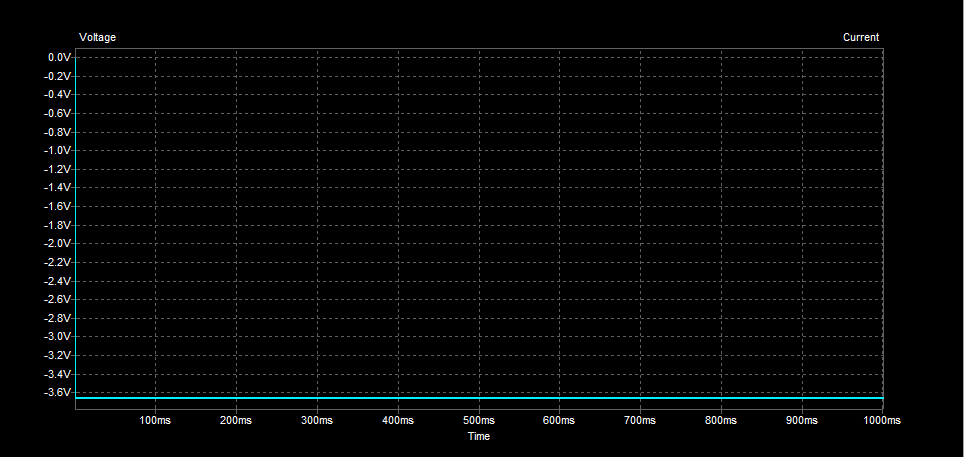
\includegraphics[width=7in]{images/simulation_sum4.png}
	\end{figure}
	\vspace{20px}
	\begin{figure}[H]
		Test 2 : a=1, b=.775v, c=.671, Competitor product output: -5.94v.
		\centering
		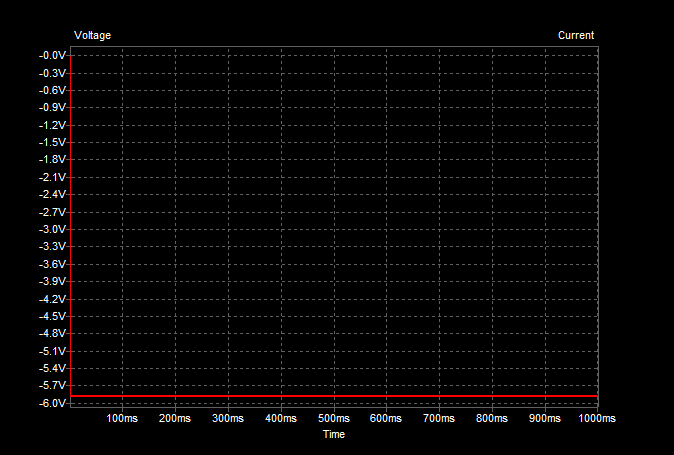
\includegraphics[width=7in]{images/simulation_sum2.png}
	\end{figure}
	\vspace{20px}
	\begin{figure}[H]
		Test 3 : a=1, b=1.004v, c=.848v, Competitor product output: -7.48v. 
		\centering
		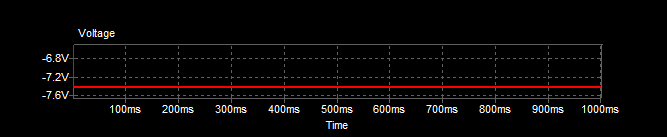
\includegraphics[width=7in]{images/simulation_sum1.png}
	\end{figure}
	
	\subsubsection*{Integrator Module}
	To test the integrator subcircuit we input a square wave on one of the inputs, expecting to get a triangle wave out. This was the case, demonstrating that the circuit functions as expected.
	\begin{figure}[H]
		\centering
		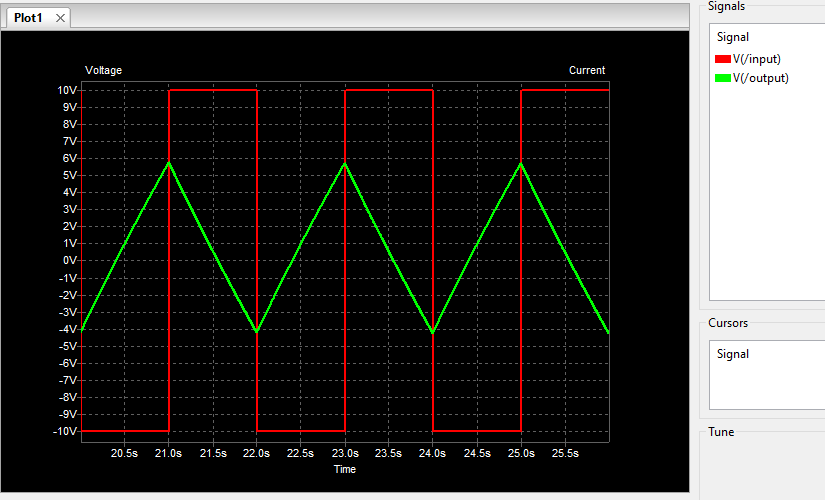
\includegraphics[width=7in]{images/simulation_integration.png}
	\end{figure}
	
	\subsection*{Design Advantages}	
	The analog computer we have designed has several advantages over the AMF Computer. The main advantage is that we cut costs by minimizing the number of materials we need to produce our computer by only including the two Op Amps. Additionally, we produced easy-to-read schematics with properly labeled pins on the Op Amp - unlike our competitor's product. Differences between our design and the competitor's design were otherwise quite limited so that they both perform the same.
	
	\subsection *{Analog vs. Digital}
	For the analog computer design, some pros include: outputs can be any real values or even irrational values like pi; the resulting voltage is instantaneously found and it can calculate high values or repetitive calculations quickly. Some cons with the analog design are: that it serves a single purpose, and it is more susceptible to noise. 
	For the digital computer design, which is more common today, the pros include: that it can be reprogrammed to perform other tasks; and fine tuning allows for less noise. The cons include: that it can only give you quantified, fixed values or approximations of values; for repeated calculations, it is harder to be processed, but due to greater advancements in processors, this is now as fast as or faster than an analog design. Overall, digital computers are more heavily used as a result of their versatility, and our boss who insists that digital is 'just a fad' will be sorely mistaken.  
	
	Our Analog Computer has several advantages over a digital equivalent. Digital devices, no matter how good, have to run at a finite sample rate and accuracy; analog computers do not have this limit. In an analog computer the results can be any real number, and are available theoretically immediately (limited by some fraction of the speed of light) while digital devices update only one discreet time per clock cycle and can only represent results to a limited number of bits of precision, perhaps to a precision of outputmax/256 or outputmax/1024. Additionally, for the specific task that our analog computer is designed for, the cost is much lower. The passive components are very cheap, while the opamps are available for about 30 cents. (The LM741 is a bad example of digital vs analog - the practical bandwidth is very limited.) Digital components for sampling the inputs and producing the outputs are many times more expensive.
	\subsection *{Conclusion}
	The tests and designs were performed without issue. There was greater error in the integrating circuit because of the input voltage drifting as we performed the test but aside from this the error was minimal. We were successfully able to design and perform simulations on the our design that performed as well as the AMF computer.
	\\
	\newpage
	\section*{Appendix A - Designing in kiCad, Simulations}
	When we were first designing our new analog computer, going off the schematic was somewhat of a challenge due to the fact that it was hand drawn. We used KiCad to design and model the schematic, and the integrating op amp was the most work to get it to operate the same as the original.
	
	
	
\end{document}
